\documentclass{article}
\usepackage{tikz}
\usepackage{xcolor}
\usepackage{mathtools}

\definecolor{darkgreen}{rgb}{0.0,0.5,0.0}
\begin{document}

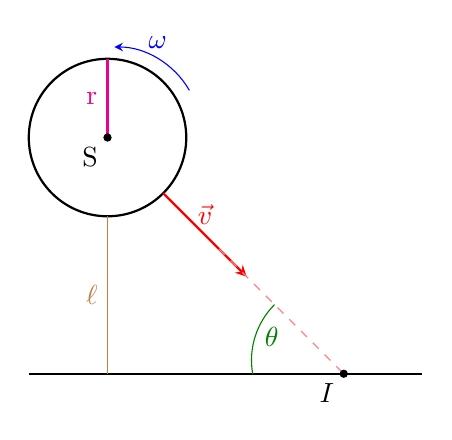
\begin{tikzpicture}
	%ball
	\draw[thick] (0,0) circle (1);
	%radius
	\draw[magenta,thick] (0,0) --node[midway,left] {r}++ (0,1);
	\node[fill=black,circle,inner sep=0pt, minimum size=3pt](s) at (0,0) {};
	%center
	\node[below left](slabel) {S};

	%speed
	\draw[red,thick,-stealth](-45:1) --node[above] {$\vec{v}$}++ (-45:1.5);
	\draw[red!50,dashed](-45:2) -- (-45:4.3);

	%graund
	\draw[thick] (-1,-3) -- (4,-3);

	%vercial length
	\draw[brown] (0,-1) --node[left] {$\ell$}++ (0,-2);

	%angle
	\node[fill=black,circle,inner sep=0pt, minimum size=3pt](naraz) at (3,-3)
	{};
	\node[below left] at (naraz) {$I$};

	\draw[darkgreen] (-45:3) arc[
			start angle = 135,
			end angle = 190,
			radius = 1,
		] node[midway,right] {$\theta$};

	%angular velocity
	\draw[blue,-stealth] (30:1.2) arc(30:90:1.1) node[midway,above] {$\omega$};
\end{tikzpicture}
\end{document}

